\section{Results Individual differences}

The secondary research question declaring the interest in investigating possible individual differences in brain activation related to sensitivity, and if the use of FSL FIX would in increase any findings. The amount positive and negative brain activation related to the sensitivity of each individual in the test population can be seen in \figref{STD_pos_ID} and \figref{STD_neg_ID} when preprocessing the data using standard preprocessing. 

\begin{figure}[H]                 
	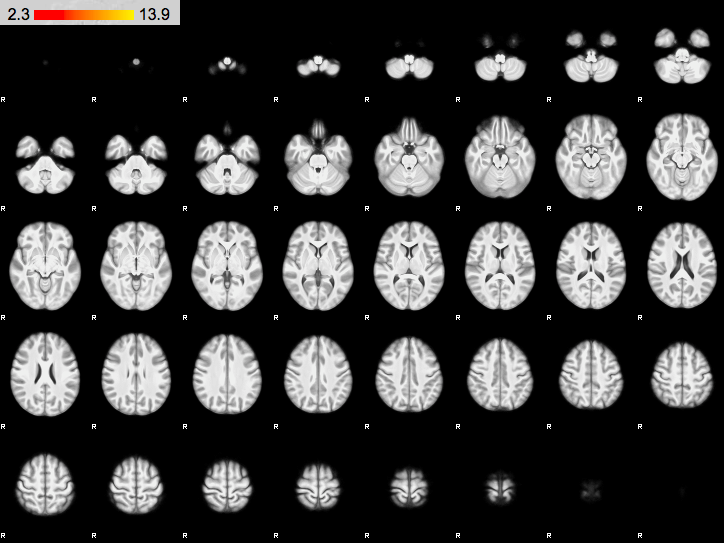
\includegraphics[width=.65\textwidth]{figures/Results/STD_pos_ID}  
	\caption{An example component of signal, which is recognizable, isolated, and not corrupted by a substantial amount of noise. In this example, the signal is characterized as a strong and fairly isolated activation mainly in the parietal lobe and some in the temporal lobe.}
	\label{STD_pos_ID} 
\end{figure}

\begin{figure}[H]                 
	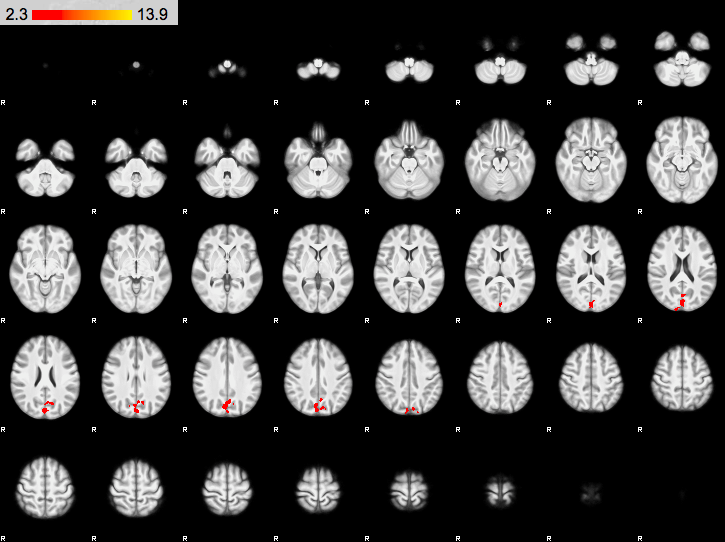
\includegraphics[width=.65\textwidth]{figures/Results/STD_neg_ID}  
	\caption{An example component of signal, which is recognizable, isolated, and not corrupted by a substantial amount of noise. In this example, the signal is characterized as a strong and fairly isolated activation mainly in the parietal lobe and some in the temporal lobe.}
	\label{STD_neg_ID} 
\end{figure}

\begin{figure}[H]                 
	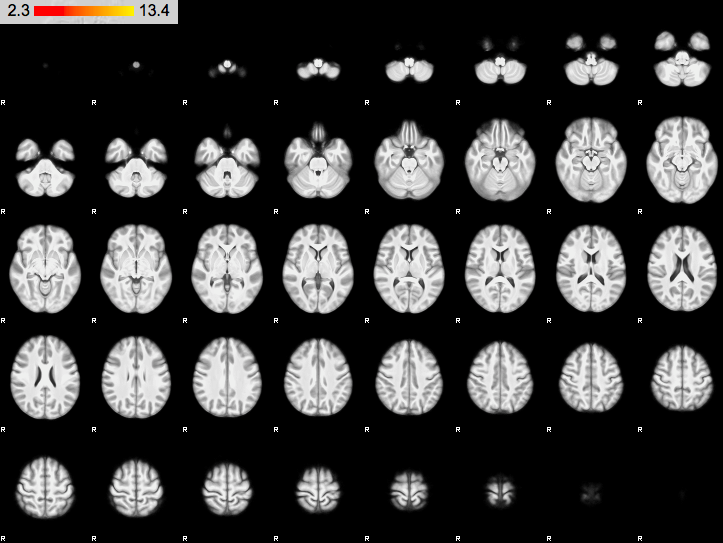
\includegraphics[width=.65\textwidth]{figures/Results/FIX_pos_ID}  
	\caption{An example component of signal, which is recognizable, isolated, and not corrupted by a substantial amount of noise. In this example, the signal is characterized as a strong and fairly isolated activation mainly in the parietal lobe and some in the temporal lobe.}
	\label{FIX_pos_ID} 
\end{figure}

\begin{figure}[H]                 
	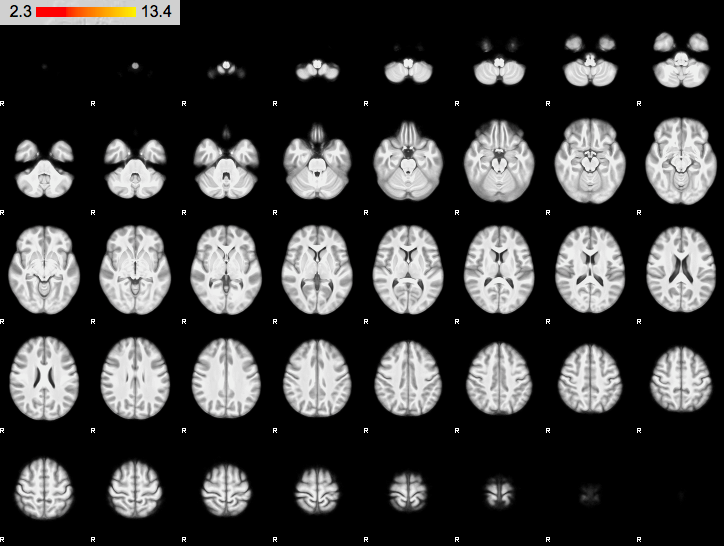
\includegraphics[width=.65\textwidth]{figures/Results/FIX_neg_ID}  
	\caption{An example component of signal, which is recognizable, isolated, and not corrupted by a substantial amount of noise. In this example, the signal is characterized as a strong and fairly isolated activation mainly in the parietal lobe and some in the temporal lobe.}
	\label{FIX_neg_ID} 
\end{figure}


















%Achieving an optimal signal to noise ratio when preprocessing task related fMRI is very desirable. The BOLD signal can be corrupted by physiological noise of non interest, subject movement and scanner artifacts. In addition, higher tesla scanners introduce the risk of more noise. A often applied method for finding noise sources is to use ICA, where the signal is broken down to components of signal and noise, which facilitates the possibility of removing those of non interest. This approach can be very time consuming on larger datasets, pushing the need for automatic noise removal algorithms.
%The aim of the project was to investigate if using the automatic de-noising tool FSL FIX would provide a greater signal to noise ratio compared to a pipeline of standard preprocessing in relation to an investigation of individual differences to a noxious heat stimuli.      